\documentclass[../../main.tex]{subfiles}

\graphicspath{{../../image/}{../../figure/}}

\begin{document}

\section{注意力}\label{section:ch12-注意力}

Transformer是深度学习领域最重要的进展之一。基于一种称为注意力（attention）的处理概念，Transformer能使网络对不同的输入赋予不同的权重，而这些加权系数本身又取决于输入值，从而捕捉到与序列数据和其他形式数据相关的强大归纳偏差。这类模型之所以叫Transformer，是因为它们能将某个表示空间中的一组向量变换成某个新空间中具有相同维度的相应向量的集合。变换旨在使新空间具有更丰富的内部表示，该表示更适合解决下游任务。对于Transformer而言，其输入可以是非结构化的向量集、有序序列或其他更一般的表示形式，从而使Transformer具有广泛的适用性。

Transformer最初是在自然语言处理（Natural Language Processing, NLP）领域引入的，这里的“自然”语言指的是像英语或汉语这样的语言，它大大超越了之前基于递归神经网络（Recurrent Neural Network, RNN）的那些最先进的方法。随后，人们发现Transformer在许多其他领域也取得了优异成果。例如，视觉Transformer在图像处理任务中的表现往往优于卷积神经网络（Convolutional Neural Network, CNN），而结合文本、图像、音频和视频等多种类型数据的多模态Transformer则是最强大的深度学习模型之一。

Transformer的一大优势在于迁移学习效果显著，所以Transformer可以在大量数据上进行训练，然后通过某种形式的微调，将经过训练的模型应用于众多下游任务。一个大规模模型随后可以进行调整以解决多个不同的任务，它就是所谓的基础模型（foundation model）。此外，Transformer可以使用无标签数据以自监督的方式进行训练（foundation model）。此外，Transformer可以使用无标签数据以自监督的方式进行训练，这对语言模型尤其有效，因为Transformer可以利用来自互联网和其他来源的海量文本。缩放假设（scaling hypothesis）认为，只要扩大模型的规模（以可学习参数的数量来衡量），并在相应的大规模数据集上进行训练，即使不改变架构，也能显著提高性能。此外，Transformer特别适用于大规模并行处理硬件，如图形处理单元（Graphics Processing Unit, GPU），从而能在合理的时间内训练出拥有万亿（$10^{12}$）规模参数的超大型神经网络语言模型。这些模型具有非凡的能力，并展现出被描述为通用人工智能早期迹象的涌现特性（Bubeck et al., 2023）。

对于初学者来说，Transformer架构可能看起来很复杂，甚至让人望而却步，因为它涉及多个不同组件的协同工作，其中各种设计构思可能看起来很随意。因此，本章将逐步全面地介绍Transformer背后的所有关键思想，并提供清晰的直观认识以引出各种元素的设计。在介绍完Transformer架构后，我们将重点介绍自然语言处理，并在最后探讨其他应用领域。

\subsection{Transformer处理}\label{subsection:ch12-Transformer处理}

虽然注意力具有非常广泛的适用性，但我们仍将以自然语言为例引出注意力的应用。请看如下两个句子：

\begin{quote}
  I swam across the river to get to the other bank.\\
  I walked across the road to get cash from the bank.
\end{quote}

“bank”一词在这两个句子中具有不同的含义。不过，这只能通过查看句子中其他词提供的上下文才能发现。我们还看到，在决定“bank”如何翻译时，有些词发挥着尤为重要的作用。在第1个句子中，“swam”和“river”两个词最能说明“bank”指的是河边；而在第2个句子中，“cash”一词最能说明“bank”指的是金融机构。我们发现，为了对“bank”进行适当的翻译，处理这样一个句子的神经网络应该关注（换句话说，更依赖于）句子中其余部分的特定词。注意力的概念如图12.1所示。

作为Transformer的核心概念，注意力最初是作为机器翻译领域递归神经网络（参见12.2.5小节）的增强版而开发的（Bahdanau, Cho, and Bengio, 2014）。不过，Vaswani et al. (2017) 后来证明，如果去除递归结构，转而只专注于注意力机制，就能显著提高性能。如今，在几乎所有应用中，基于注意力的Transformer已完全取代递归神经网络。

在讨论自然语言处理时，我们将了解如何使用词嵌入（word embedding）将词投射到嵌入空间中的向量。这些向量可用作后续神经网络处理的输入。这些词嵌入可以捕捉到基本的语义属性，例如，将具有相似含义的词映射到嵌入空间中的邻近位置。这种嵌入的一个特点是，给定的词总是被映射到同一个嵌入向量。Transformer可以视为一种更丰富的嵌入形式，其中一个给定向量被映射到一个依赖序列中其他向量的位置。因此，上述示例中代表“bank”的向量可以映射到两个不同句子的新嵌入空间中的不同位置。例如，在第1个句子中，变换后的表示可能会将“bank”在嵌入空间中靠近“water”；而在第2个句子中，变换后的表示可能会将“bank”放在靠近“money”的位置。

下面我们以蛋白质建模为例来说明注意力的重要性。我们可以把蛋白质看作由分子单元（称为氨基酸）组成的一维序列。一个蛋白质可能由数百或数千个这样的分子单元组成，每个分子单元由22种可能性中的一种给定。在活细胞中，蛋白质折叠成三维结构，一维序列中互相远离的氨基酸可以在三维空间中变得接近，从而产生相互作用。Transformer模型允许这些互相远离的氨基酸相互“关注”，从而大大提高了三维结构建模的准确性（Vig et al., 2020）。

在清楚地了解Transformer的工作原理之前，我们必须准确地使用符号。我们将按照标准惯例，将数据向量组合成一个$N\times D$维的矩阵$\mathbf{X}$，其中第$n$行是token向量$\mathbf{x}_n$，$n=1,\cdots,N$，如图12.3所示。请注意，该矩阵代表一组输入token，而在大多数应用中，我们需要一个包含多组token的数据集，例如每个词都是由一个token表示的独立文本段落。

Transformer的输入数据是一组$D$维向量$\{\mathbf{x}_n\}$，其中$n=1,\cdots,N$。我们将这些数据向量称为token，一个token可能对应句子中的一个词、图像中的一个小块或者蛋白质中的一个氨基酸。token中的元素$x_{ni}$称为特征。稍后我们将了解如何为自然语言数据和图像构建这些token向量。Transformer的一个强大特性是，我们无须设计新的网络架构来处理不同类型的数据，而只需要将数据变量组合成一组联合token即可。

Transformer的基本构件是一个函数，用于将数据矩阵作为输入并创建一个具有相同维度的变换矩阵$\bar{\mathbf{X}}$作为输出。我们可以写下该函数，形式如下：

\begin{align}
  \bar{\mathbf{X}} = \mathrm{TransformerLayer}[\mathbf{X}]
  \label{align:ch12-Transformer层}
\end{align}

其中$\bar{\mathbf{X}}$的第$n$行代表变换后的数据向量$\bar{\mathbf{x}}_n$。然后，我们可以连续叠加多个Transformer层来构建能够学习丰富内部表示的深度网络。每个Transformer层都有自己的权重和偏置，可以通过梯度下降法使用适当的损失函数进行学习，这将在本章后续部分（参见12.3节）详细讨论。Transformer层本身包含两个阶段。在实现注意力机制的第一阶段，将数据矩阵各列中不同token向量的相应特征混合在一起；第二阶段则独立作用于每一行，并对每个token向量中的特征进行变换。

\subsection{注意力系数}\label{subsection:ch12-注意力系数}

假设嵌入空间中有一组输入token $\mathbf{x}_1,\cdots,\mathbf{x}_N$，我们希望将它们映射到另一组具有相同数量token但位于一个新嵌入空间的$\mathbf{y}_1,\cdots,\mathbf{y}_N$，这一新的嵌入空间能捕捉到更丰富的语义结构。考虑一个特定的输出向量$\mathbf{y}_n$。$\mathbf{y}_n$的值不仅取决于相应的输入向量$\mathbf{x}_n$，还取决于集合中所有其他的输入向量。凭借注意力，对于那些在确定$\mathbf{y}_n$的修正表示中发挥特别重要作用的输入向量$\mathbf{x}_m$来说，这种依赖性应该更强。实现这一目标的简单方法是将每个输出向量$\mathbf{y}_n$定义为输入向量$\mathbf{x}_1,\cdots,\mathbf{x}_N$与加权系数$a_{nm}$的线性组合：

\begin{align}
  \mathbf{y}_n = \sum_{m=1}^{N} a_{nm}\,\mathbf{x}_m
  \label{align:ch12-注意力加权}
\end{align}

其中，$a_{nm}$称为注意力权重（attention weight），又称注意力系数或权重系数。对于对输出$\mathbf{y}_n$影响较小的输入token，注意力系数应接近于零；而对于对输出$\mathbf{y}_n$影响最大的输入token，注意力系数应最大。因此，我们限制注意力系数为非负值，以避免出现一个注意力系数变大为正值，而另一个注意力系数补偿变小为负值的情况。我们还希望确保如果一个输出对某一特定输入给予更多注意力，则应该以减少对其他输入的注意力为代价，因此我们限制注意力系数的总和为1：加权系数必须满足以下两个约束条件：

\begin{align}
  a_{nm} \geq 0
  \label{align:ch12-系数非负}
\end{align}

\begin{align}
  \sum_{m=1}^{N} a_{nm} = 1
  \label{align:ch12-系数归一}
\end{align}

这意味着每个注意力系数都在$0\leq a_{nm}\leq 1$的范围内，因此这些注意力系数定义了一个“单位分解”（见习题12.1）。在$a_{nm}=1$且当$n=m$时$a_{nm}=0$的特殊情况下，由于$\mathbf{y}_n=\mathbf{x}_n$，输入向量在变换后保持不变。一般来说，输出向量$\mathbf{y}_n$是输入向量的混合体，其中一些输入向量的权重系数高于其他输入向量。

请注意，我们为每个输出向量$\mathbf{y}_n$设置了一组不同的系数，而约束条件[式~\eqref{align:ch12-系数非负}和式~\eqref{align:ch12-系数归一}]分别适用于每个$n$值。这些系数取决于输入数据，后续我们将展示如何计算它们。

\subsection{自注意力}\label{subsection:ch12-自注意力}

接下来的问题是如何确定权重系数$a_{nm}$。在展开详细讨论之前，我们不妨先了解一下信息检索领域的一些术语。以通过线上电影流媒体服务选择观看哪部电影为例。一种方法是将每部电影与一系列属性关联起来，这些属性描述了电影的类型（喜剧、动作片等）、主演姓名、片长等。用户可以通过目录搜索找到自己喜欢看的电影。我们可以将每部电影的属性编码成一个称为键（key）的向量，从而将该过程自动化。相应的电影文件本身叫作值（value）。同样，用户也可以为所需属性提供自己的个人值向量，我们称之为查询（query）。然后，线上电影流媒体服务可以将查询向量与所有键向量作比较，从而找出最佳匹配，并以值文件的形式将相应的电影发送给用户。用用户所“关注”的特定电影，其键向量最匹配于用户的查询向量。这可以视为硬注意力（hard attention）的一种形式，其会返回一个单一值向量。对于Transformer，我们可以将其泛化到软注意力（soft attention）中，即使用连续变量来度量查询和键之间的匹配程度，然后使用这些变量来权衡值向量对输出的影响。这也将确保Transformer函数是可微分的，从而可以通过梯度下降法进行训练。

参照信息检索的方法，我们可以将每个输入$\mathbf{x}_n$视为一个值向量，用来创建输出token。我们还可以直接使用$\mathbf{x}_n$作为输入token $n$的键向量。这就好比用电影本身来概括电影的特点。最后，我们可以使用$\mathbf{x}_n$作为输出$\mathbf{y}_n$的查询向量，然后将其与每个键向量作比较。要想知道$\mathbf{x}_n$代表的token与$\mathbf{x}_m$代表的token有多大的相似度，我们需要计算出这些向量的相似度。度量向量相似度的一种简单方法是求它们的点积$\mathbf{x}_n^{\mathsf{T}}\mathbf{x}_m$。为了施加约束条件[式~\eqref{align:ch12-系数非负}和式~\eqref{align:ch12-系数归一}]，使用softmax函数变换点积（参见5.3节），以定义权重系数$a_{nm}$：

\begin{align}
  a_{nm} = \frac{\exp\left(\mathbf{x}_n^{\mathsf{T}}\mathbf{x}_m\right)}{\sum_{m'=1}^{N}\exp\left(\mathbf{x}_n^{\mathsf{T}}\mathbf{x}_{m'}\right)}
  \label{align:ch12-点积注意力系数}
\end{align}

请注意，在这种情况下，softmax函数不存在概率解释，它只是用来对注意力权重进行适当的归一化。

因此，总的来说，每个输入向量$\mathbf{x}_m$都是通过形式为式~\eqref{align:ch12-注意力加权}的输入向量线性组合而转换为相应的输出向量$\mathbf{y}_n$的，其中应用于输入向量$\mathbf{x}_m$的权重系数$a_{nm}$由softmax函数给出[式~\eqref{align:ch12-点积注意力系数}]，该softmax函数是根据输入$n$的查询向量$\mathbf{x}_n$与输入$m$相关的键向量$\mathbf{x}_m$之间的点积$\mathbf{x}_n^{\mathsf{T}}\mathbf{x}_m$进行定义的。请注意，如果所有输入向量都是正交的，那么每个输出向量都等于相应的输入向量，从而在$m=1,\cdots,N$的情况下，$\mathbf{y}_m=\mathbf{x}_m$（见习题12.3）。

我们可以使用数据矩阵$\mathbf{X}$和类似的$N\times D$输出矩阵$\mathbf{Y}$（其行由$\mathbf{y}_m$给出）将式~\eqref{align:ch12-注意力加权}用矩阵符号写出：

\begin{align}
  \mathbf{Y} = \mathrm{Softmax}\left[\mathbf{X}\mathbf{X}^{\mathsf{T}}\right]\mathbf{X}
  \label{align:ch12-点积自注意力矩阵}
\end{align}

其中，$\mathrm{Softmax}[\cdot]$是一个算子，作用是取矩阵$\mathbf{L}$中每个元素的指数，然后将每一行独立归一化，使它们的和为1。这个过程叫作自注意力（self-attention），因为我们使用相同的序列来确定查询、键和值。在后续内容中，我们还会遇到这种注意力的变体。此外，由于查询向量和键向量之间的相似度度量是由点积给出的，因此这个过程又叫作点积自注意力（dot-product self-attention）。

\subsection{网络参数}\label{subsection:ch12-网络参数}

目前，由于没有可调整的参数，从输入向量$\mathbf{x}_n$到输出向量$\mathbf{y}_n$的变换是固定的，且不具备从数据中学习的能力。此外，token向量$\mathbf{x}_n$的每个特征值在确定注意力系数时发挥相同的作用，而我们希望网络在确定token相似度时能够灵活地将注意力更多地集中在某些特征上。通过定义由原始向量的线性变换给出的修正特征向量，我们可以解决这两个问题：

\begin{align}
  \tilde{\mathbf{X}} = \mathbf{X}\mathbf{U}
  \label{align:ch12-特征线性变换}
\end{align}

其中$\mathbf{U}$是可学习权重参数的$D\times D$矩阵，类似于标准神经网络中的“层”，从而得到一个修正后的变换，其形式为

\begin{align}
  \mathbf{Y} = \mathrm{Softmax}\left[\tilde{\mathbf{X}}\tilde{\mathbf{X}}^{\mathsf{T}}\right]\tilde{\mathbf{X}}
  \label{align:ch12-可学习点积注意力}
\end{align}

虽然这种方法更灵活，但它有一个特性，即如下矩阵是对称的：

\begin{align}
  \tilde{\mathbf{X}}\tilde{\mathbf{X}}^{\mathsf{T}} = \mathbf{X}\mathbf{U}\mathbf{U}^{\mathsf{T}}\mathbf{X}^{\mathsf{T}}
\end{align}

虽然softmax函数意味着得到的注意力权重矩阵本身并不对称，但我们可以通过允许查询和键具有独立参数来创建一个更加灵活的模型。然而，式~\eqref{align:ch12-可学习点积注意力}使用相同的参数矩阵$\mathbf{U}$来定义值向量和注意力系数，这似乎又是一个不受欢迎的限制。此外，注意力权重矩阵本身并不对称，因为我们可能会认为“斧头”与“工具”的关联性很强，因为每一把斧头都是一个工具；而“工具”与“斧头”的关联性很弱，因为除了斧头，还有许多其他种类的工具。而我们希望注意力机制支持明显的不对称。

通过定义单独的查询矩阵、键矩阵和值矩阵，并让每个矩阵都有自己独立的线性变换，我们可以克服这些限制：

\begin{align}
  \mathbf{Q} = \mathbf{X}\mathbf{W}^{(Q)}
  \label{align:ch12-查询矩阵}
\end{align}

\begin{align}
  \mathbf{K} = \mathbf{X}\mathbf{W}^{(K)}
  \label{align:ch12-键矩阵}
\end{align}

\begin{align}
  \mathbf{V} = \mathbf{X}\mathbf{W}^{(V)}
  \label{align:ch12-值矩阵}
\end{align}

其中，权重矩阵$\mathbf{W}^{(Q)}$、$\mathbf{W}^{(K)}$和$\mathbf{W}^{(V)}$表示在训练最终的Transformer架构时将学习到的参数。矩阵$\mathbf{W}^{(K)}$的维度为$D\times D_k$，其中$D_k$是键向量的长度。矩阵$\mathbf{W}^{(Q)}$的维度为$D\times D_k$必须与矩阵$\mathbf{K}$的维度相同，因为只有这样才能在查询向量和键向量之间形成点积。为此，可以设置$D_q=D_k$。同样，$\mathbf{W}^{(V)}$是一个维度为$D\times D_v$的矩阵，其中$D_v$是输出向量的长度。如果设置$D_v=D$，使输出表示和输入表示具有相同的维度，则有助于加入残差连接，我们稍后将对此进行讨论。此外，如果每个层的维度相同，则多个Transformer层可以叠加在一起（参见12.1.7小节）。通过对式~\eqref{align:ch12-可学习点积注意力}进行泛化，我们可以得到

\begin{align}
  \mathbf{Y} = \mathrm{Softmax}\left[\mathbf{Q}\mathbf{K}^{\mathsf{T}}\right]\mathbf{V}
  \label{align:ch12-通用注意力}
\end{align}

其中矩阵$\mathbf{Q}\mathbf{K}^{\mathsf{T}}$的维度为$N\times N$，且矩阵$\mathbf{Y}$的维度为$N\times D_v$。矩阵$\mathbf{Q}\mathbf{K}^{\mathsf{T}}$的计算如图12.4所示，而矩阵$\mathbf{Y}$的计算如图12.5所示。

实际上，我们还可以在这些线性变换中加入偏置参数。不过，偏置参数也可以包含在权重矩阵中，就像我们对标准神经网络所做的那样（参见6.2.1小节），方法是在数据矩阵$\mathbf{X}$中增加一列1，然后在权重矩阵中增加额外一行参数来表示偏置。自此，我们将把偏置参数视为隐参数，以免混淆符号。

\subsection{缩放自注意力}\label{subsection:ch12-缩放自注意力}

我们还可以对自注意力层进行最后一次改进。回想一下，当输入量较大时，softmax函数的梯度会呈指数减小，就像tanh函数或逻辑斯谛sigmoid函数一样。为了避免出现这种情况，我们可以在应用softmax函数之前重新缩放查询向量和键向量的点积。为了得到合适的缩放结果，请注意，如果查询向量和键向量的元素都是均值为0且方差为单位方差的独立随机数，则点积的方差就是$D_k$（见习题12.4）。因此，我们使用$D_k$的平方根所给出的标准差对softmax的参数进行归一化处理，从而注意力层的输出形式为

\begin{align}
  \mathrm{Attention}(\mathbf{Q},\mathbf{K},\mathbf{V}) = \mathrm{Softmax}\left[\frac{\mathbf{Q}\mathbf{K}^{\mathsf{T}}}{\sqrt{D_k}}\right]\mathbf{V}
  \label{align:ch12-缩放点积注意力}
\end{align}

这就是所谓的缩放点积自注意力（scaled dot-product self-attention），也是自注意力神经网络层的最终形式。这一层的结构如图12.6所示，算法过程见算法12.1。

\subsection{多头注意力}\label{subsection:ch12-多头注意力}

注意力层允许输出向量关注输入向量的依赖数据模式，称作注意力头（attention head）。然而，可能同时存在多种相关的注意力模式。例如，在自然语言中，有些注意力模式可能与时态有关，而另一些注意力模式则可能与词汇有关。使用单一注意力头会导致这些效应的平均化。对此，我们可以并行使用多个注意力头。这些注意力头由结构相同的单个注意力头的副本组成，具有独立的可学习参数，用于控制查询矩阵、键矩阵和值矩阵的计算。这类似于在卷积网络的每一层中使用多个不同的过滤器。

假设我们有$H$个注意力头，以$h=1,\cdots,H$进行编号，形式为

\begin{align}
  \mathbf{H}_h = \mathrm{Attention}(\mathbf{Q}_h,\mathbf{K}_h,\mathbf{V}_h)
  \label{align:ch12-单头注意力}
\end{align}

其中$\mathrm{Attention}(\cdot,\cdot,\cdot)$由式~\eqref{align:ch12-缩放点积注意力}给出，使用如下方法为每个注意力头定义单独的查询矩阵、键矩阵和值矩阵：

\begin{align}
  \mathbf{Q}_h = \mathbf{X}\mathbf{W}_h^{(Q)},\qquad
  \mathbf{K}_h = \mathbf{X}\mathbf{W}_h^{(K)},\qquad
  \mathbf{V}_h = \mathbf{X}\mathbf{W}_h^{(V)}
  \label{align:ch12-多头QKV}
\end{align}

首先将各个注意力头合并成一个单一矩阵，然后使用矩阵$\mathbf{W}^{(O)}$对结果进行线性变换，从而得到一个合并输出，形式为

\begin{align}
  \mathbf{Y}(\mathbf{X}) = \mathrm{Concat}\left[\mathbf{H}_1,\cdots,\mathbf{H}_H\right]\mathbf{W}^{(O)}
  \label{align:ch12-多头注意力合并}
\end{align}

多头注意力网络的结构如图12.7所示，算法过程见算法12.2。

每个矩阵$\mathbf{H}_h$的维度为$N\times D_v$，因此合并矩阵的维度为$N\times HD_v$。在使用维度为$HD_v\times D$的线性矩阵$\mathbf{W}^{(O)}$进行变换后，最终得到维度为$N\times D$的输出矩阵$\mathbf{Y}$，它与原始输入矩阵$\mathbf{X}$的维度相同。矩阵$\mathbf{W}^{(O)}$的元素是在训练阶段与查询矩阵、键矩阵和值矩阵一起学习的。通常情况下，$D_v$选择为与$D/H$相等，从而使得到的合并矩阵的维度为$N\times D$。图12.8展示了多头注意力层的信息流。

请注意，前文给出的多头注意力表述与研究文献中使用的表述相同，我们在每个注意力头的$\mathbf{W}^{(V)}$矩阵与输出矩阵$\mathbf{W}^{(O)}$的连续乘法中包含了一些冗余。在消除这些冗余后，多头自注意力层就可以写成每个注意力头的贡献之和（见习题12.5）。

\subsection{Transformer层}\label{subsection:ch12-Transformer层}

多头自注意力构成了Transformer网络的核心架构元素。我们知道，神经网络从深度结构中获益匪浅，因此我们希望将多个自注意力层堆叠在一起。为了提高训练效率，我们可以引入绕过多头结构的残差连接（参见9.5节）。为此，我们要求输出维度与输入维度相同（参见7.4.3小节）。然后进行层归一化（layer normalization）（Ba, Kiros, and Hinton, 2016），从而提高训练效率。由此产生的变换可以写成

\begin{align}
  \mathbf{Z} = \mathrm{LayerNorm}\left[\mathbf{Y}(\mathbf{X}) + \mathbf{X}\right]
  \label{align:ch12-注意力残差LN}
\end{align}

其中$\mathbf{Y}$由式~\eqref{align:ch12-多头注意力合并}定义。有时，层归一化会被预归一化取代，即层归一化在多头注意力之前而不是之后进行，因为这可以带来更有效的优化。在这种情况下，我们得出

\begin{align}
  \mathbf{Z} = \mathbf{Y}(\mathbf{X}') + \mathbf{X},\qquad \text{其中}\quad \mathbf{X}' = \mathrm{LayerNorm}\left[\mathbf{X}\right]
  \label{align:ch12-预归一化注意力}
\end{align}

此外，这些值向量是输入向量的线性函数，因此我们可以看到，注意力层的输出受限于输入的线性组合。非线性通过注意力权重引入，因此输出将通过softmax函数非线性地依赖于输入，但输出向量仍然受限于输入向量所跨的子空间，这限制了注意力层的表达能力。我们可以使用一个标准的非线性神经网络（有$D$个输入和$D$个输出）对每一层的输出进行后处理，用$\mathrm{MLP}[\cdot]$表示“多层感知机”，从而提高Transformer的灵活性。例如，这可能包括一个具有ReLU隐藏单元的两层全连接网络。当我们这样做时，需要保持Transformer处理不同长度序列的能力。为此，我们需要对每个输出向量（与$\mathbf{Z}$的行相对应）应用相同的共享网络。同样，也可以通过使用残差连接来改进该神经网络层。它还包括层归一化，从而Transformer层的最终输出形式为

\begin{align}
  \mathbf{X}' = \mathrm{LayerNorm}\left[\mathrm{MLP}[\mathbf{Z}] + \mathbf{Z}\right]
  \label{align:ch12-FFN残差LN}
\end{align}

在这种情况下，Transformer层的最终输出形式为

\begin{align}
  \mathbf{X}' = \mathrm{MLP}[\mathbf{Z}'] + \mathbf{Z},\qquad \text{其中}\quad \mathbf{Z}' = \mathrm{LayerNorm}\left[\mathbf{Z}\right]
  \label{align:ch12-预归一化FFN}
\end{align}

这就产生了Transformer层的整体架构，如图12.9所示，算法过程见算法12.3。

\begin{figure}[htbp]
  \centering
  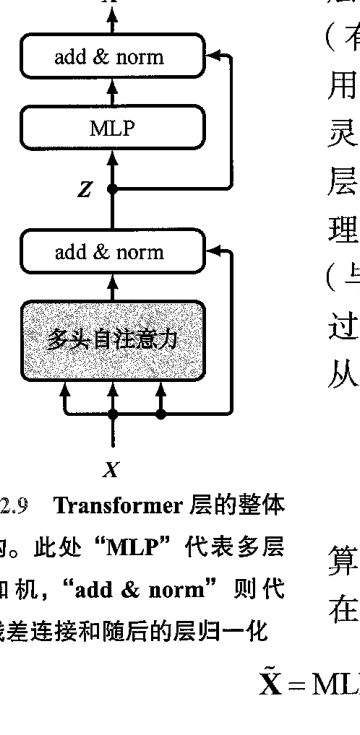
\includegraphics[width=0.45\textwidth]{ch12-fig346-transformer-layer.png}
  \caption{Transformer层的整体架构。此处“MLP”代表多层感知机，“add \& norm”则代表残差连接和随后的层归一化。}
  \label{figure:ch12-Transformer层架构}
\end{figure}同样，我们也可以使用预归一化。在典型的Transformer模型中，有多个这样的层叠加在一起。虽然不同层之间不共享权重和偏置，但各层通常具有相同的结构。

\subsection{计算复杂性}\label{subsection:ch12-计算复杂性}

到目前为止我们所讨论的注意力层包含一个向量集（其中有$N$个向量，每个向量的长度为$D$），我们将它映射到了另一个具有相同维度的向量集（其中也有$N$个向量）。因此，输入和输出的总维度均为$ND$。如果我们使用标准的全连接神经网络将输入值映射到输出值，就会有$O(N^2 D^2)$个独立参数。同样，计算通过这样一个网络进行一次前向传递的成本也是$O(N^2 D^2)$。

在注意力层中，矩阵$\mathbf{W}^{(Q)}$、$\mathbf{W}^{(K)}$和$\mathbf{W}^{(V)}$在输入token之间共享，因此独立参数的数量为$O(D^2)$，这里假设$D_q\approx D_v=D$。由于有$N$个输入token，在自注意力层中计算点积的步骤数为$O(N^2 D)$。我们可以把自注意力层看作一个稀疏矩阵，其中的参数在矩阵的特定块之间共享。随后的神经网络层（它有$D$个输入和$D$个输出）的成本为$O(D^2)$。由于它在token之间共享，其复杂度与$N$成线性关系，因此这一层的总成本为$O(ND^2)$。

根据$N$和$D$的相对大小，Transformer层或多层感知机层有可能支配计算成本。与全连接网络相比，Transformer层的计算效率更高。Transformer架构的许多变体已被提出（Lin et al., 2021; Phuong and Hutter, 2022），包括旨在提高效率的修正版（Tay et al., 2020）。

\subsection{位置编码}\label{subsection:ch12-位置编码}

在Transformer架构中，矩阵$\mathbf{W}^{(Q)}$、$\mathbf{W}^{(K)}$和$\mathbf{W}^{(V)}$由输入的所有token共用。同样，紧随其后的神经网络（前馈神经网络）也由输入的所有token共用。因此，Transformer具有这样的特性，即对输入token（也就是$\mathbf{X}$的行）进行排序会导致输出矩阵$\bar{\mathbf{X}}$的行也被排序。换句话说，Transformer在输入排列方面是等变化的（equivariant）。网络架构中的参数共享有利于Transformer的大规模并行处理，也使网络能够像学习短距离依赖关系一样有效地学习远距离依赖关系。然而，当我们考虑序列数据（如自然语言中的词）时，不依赖token顺序就成了一个主要的限制，因为Transformer学习到的表示法将与输入token的顺序无关。句子“The food was bad, not good at all”和“The food was good, not bad at all”包含相同的token，但由于token的排序不同，这两个句子的含义也截然不同。显然，token顺序对于包括自然语言处理在内的大多数顺序处理任务至关重要，因此我们需要找到一种方法来将有关token顺序的信息注入网络。

由于想要保留精心构建的注意力层的强大特性，因此我们希望在数据中对token顺序进行编码，而不是在网络架构中表示token顺序。为此，我们将构建一个与每个输入位置$n$相关的位置编码向量$\mathbf{r}_n$，然后将其与相关输入token的嵌入向量$\mathbf{x}_n$结合起来。增加所有后续注意力空间的维度，进而显著增加计算成本。相反，我们可以简单地将位置向量加到token向量上，从而得出

\begin{align}
  \tilde{\mathbf{x}}_n = \mathbf{x}_n + \mathbf{r}_n
  \label{align:ch12-位置编码相加}
\end{align}

这就要求位置编码向量的维度与token嵌入向量的维度相同。

接下来的任务是构建嵌入向量$\mathbf{r}_n$。一种简单的方法是为每个位置关联一个整数。但这样做的问题是，数值的大小会无限制地增加，因此可能会严重破坏嵌入向量。此外，对于比训练时所用输入序列更长的新输入序列，它可能无法很好地泛化，因为这些输入序列涉及的编码值将超出训练时所用编码值的范围。我们也可以为序列中的每个token分配一个介于0和1之间的数字，从而保持表示法的有界性。然而，这种表示法对于特定位置并不是唯一的，因为它取决于整个序列的长度。

理想的位置编码应该为每个位置提供唯一的表示，其应该是有界的，能泛化为较长的序列，且应该有一致的方法来表示任意两个输入向量之间的步数，而不管它们的绝对位置如何，因为token的相对位置往往比绝对位置更重要。位置编码的方法有很多 (Dutker, Schmitt, and Sch\"utze, 2021)。在此，我们介绍一种由Vaswani et al. (2017)引入的基于正弦函数的技术。对于给定的位置$n$，相关的编码向量具有组件$r_{ni}$，其计算公式为

\begin{align}
  r_{n,\,2i} = \sin\left(\frac{n}{10000^{2i/D}}\right),\qquad
  r_{n,\,2i+1} = \cos\left(\frac{n}{10000^{2i/D}}\right)
  \label{align:ch12-正弦位置编码}
\end{align}

当$i$是偶数时取第一式，当$i$是奇数时取第二式。这种编码的特点是，向量$\mathbf{r}_n$的元素都位于$(-1,1)$范围内。这不禁让人联想到二进制数的表示方法，最低阶位高频率地交替出现，而随后的位则以逐渐降低的频率交替出现。如图12.10(a)所示，嵌入向量$\mathbf{r}_n$的元素由一系列波长逐渐增大的正弦和余弦函数给出。

式~\eqref{align:ch12-正弦位置编码}给出的正弦表示法有一个很好的特性，即对于任何固定偏移$k$，位置$n+k$处的编码可以表示为位置$n$处编码的线性组合，其中系数不取决于绝对位置，而只取决于$k$值（见习题12.10）。因此，网络应该能够学会关注相对位置。请注意，这一特性要求编码同时使用正弦和余弦函数。不过，对于式~\eqref{align:ch12-正弦位置编码}来说，向量元素是连续变量而非二进制变量。位置编码向量的热图说明见图12.10(b)。

另一种常用的位置表示方法是使用习得的位置编码。这是通过在每个token位置设置一个权重向量来实现的，该权重向量可在训练过程中与模型的其他参数共同学习，从而避免使用人工表示法。由于token位置之间不共享参数，因此token在排列时不再是不变的，而这正是位置编码的目的。不过，这种方法并不符合前述对较长的输入序列进行泛化的标准，因为训练过程中没有出现过的位置编码未经训练。因此，当输入序列的长度在训练和推理过程中都相对固定时，这种方法通常最适用。

\end{document}
